\documentclass[10pt,oneside,onecolumn,letterpaper]{article}
\usepackage{graphicx}
\usepackage{xcolor}
\usepackage[hidelinks]{hyperref}
\usepackage{booktabs}
\usepackage{adjustbox}

\usepackage[top=.5in, bottom=1in, left=.5in, right=.7in]{geometry}

\usepackage{fontspec}
\setmainfont{Arial}

\begin{document}

%%
% THIS IS THE HEADER
%%
\noindent\colorbox{black}{
\begin{minipage}[c]{.99\linewidth}
  \vspace{.4cm}
  \Large{\color{white}{\textbf{\hspace{.3cm}University of Massachusetts Boston}}}
  \begin{flushright}
      \vspace{-1.2cm}
      
\includegraphics[width=3cm]{gfx/cs460.png}
    \end{flushright}
  \end{minipage}
  }

  %%
  % CONTENT STARTS HERE
  %%

  \vspace{.5cm} % add some space

  \noindent\textbf{CS460 Fall 2019} \\
  \textbf{Name:} Jared Barresi \\
  \textbf{Student ID:} 00974358 \\
  \textbf{Due Date:} 09/09/2019

  \section*{Assignment 1: Intro}

  \textbf{Describe your favorite WebGL demo.}

  \vspace{.5cm} % add some space

  \noindent My favorite demo is .... (\url{https://ADDLINK}). The authors show ....

  \vspace{.5cm} % add some space

  \noindent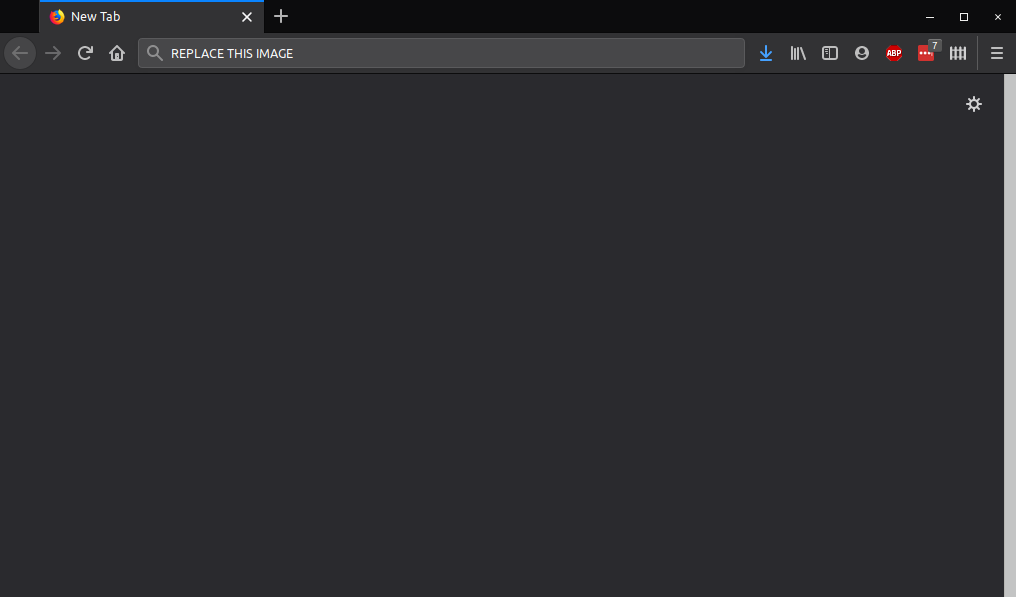
\includegraphics[width=\textwidth]{gfx/empty_browser.png}

  \vspace{.5cm} % add some space

  \noindent\textbf{Technologies used:}

  \begin{itemize}
      \item HTML/CSS/JavaScript
      \item Three.js
      \item ...
  \end{itemize}

  \noindent\textbf{Bonus:} If possible, try to host the project as your own Github repository and make it accessible via Github pages. Please make sure to credit the original authors. Then, link the repository here: \url{https://ADDLINK}

  \end{document}
